
\documentclass[DIV=calc, paper=a4, fontsize=11pt, twocolumn, spanish]{scrartcl}	 % A4 paper and 11pt font size

\usepackage{lipsum} % Used for inserting dummy 'Lorem ipsum' text into the template
\usepackage[protrusion=true,expansion=true]{microtype} % Better typography
\usepackage{amsmath,amsfonts,amsthm} % Math packages
\usepackage[svgnames]{xcolor} % Enabling colors by their 'svgnames'
\usepackage[hang, small,labelfont=bf,up,textfont=it,up]{caption} % Custom captions under/above floats in tables or figures
\usepackage{booktabs} % Horizontal rules in tables
\usepackage{fix-cm}	 % Custom font sizes - used for the initial letter in the document
\usepackage[spanish]{babel}
\selectlanguage{spanish}
\usepackage[utf8]{inputenc}
\usepackage{graphicx}

\usepackage{sectsty} % Enables custom section titles
\allsectionsfont{\usefont{OT1}{phv}{b}{n}} % Change the font of all section commands

\usepackage{fancyhdr} % Needed to define custom headers/footers
\pagestyle{fancy} % Enables the custom headers/footers
\usepackage{lastpage} % Used to determine the number of pages in the document (for "Page X of Total")

% Headers - all currently empty
\lhead{}
\chead{}
\rhead{}

% Footers
\lfoot{}
\cfoot{}
\rfoot{\footnotesize Page \thepage\ of \pageref{LastPage}} % "Page 1 of 2"

\renewcommand{\headrulewidth}{0.0pt} % No header rule
\renewcommand{\footrulewidth}{0.4pt} % Thin footer rule

\usepackage{lettrine} % Package to accentuate the first letter of the text
\newcommand{\initial}[1]{ % Defines the command and style for the first letter
\lettrine[lines=3,lhang=0.3,nindent=0em]{
\color{DarkGoldenrod}
{\textsf{#1}}}{}}

%----------------------------------------------------------------------------------------
%	TITLE SECTION
%----------------------------------------------------------------------------------------

\usepackage{titling} % Allows custom title configuration

\newcommand{\HorRule}{\color{DarkGoldenrod} \rule{\linewidth}{1pt}} % Defines the gold horizontal rule around the title

\pretitle{\vspace{-30pt} \begin{flushleft} \HorRule \fontsize{35}{35} \usefont{OT1}{phv}{b}{n} \color{DarkRed} \selectfont} % Horizontal rule before the title

\title{Dilatación térmica del agua} % Your article title

\posttitle{\par\end{flushleft}\vskip 0.2em} % Whitespace under the title

\preauthor{\begin{flushleft}\large \lineskip 0.5em \usefont{OT1}{phv}{b}{sl} \color{DarkRed}} % Author font configuration

\author{Sebastián Valencia, } % Your name

\postauthor{\footnotesize \usefont{OT1}{phv}{m}{sl} \color{Black} % Configuration for the institution name
Universidad de los Andes \\ 201111578

\par\end{flushleft}\HorRule} % Horizontal rule after the title



\date{} % Add a date here if you would like one to appear underneath the title block

%----------------------------------------------------------------------------------------

\begin{document}

\maketitle % Print the title

\thispagestyle{fancy} % Enabling the custom headers/footers for the first page 

%----------------------------------------------------------------------------------------
%	ABSTRACT
%----------------------------------------------------------------------------------------

% The first character should be within \initial{}
\initial{E}\textbf{l agua, al igual que los sólidos, está sujetos a transformaciones físicas y químicas al experimentar variaciones de temperatura. La dilatación térmica del agua, es un fenómeno físico bien entendido y estudiado. Es necesario confirmar la intuición física haciendo uso de la experimentación. En la practica de laboratorio, se pretende estudiar de manera experimental la dilatación térmica del agua, de esta forma, se confirma la intuición física y se  solidifica el entendimiento del método científico y la importancia de la experimentación}

%----------------------------------------------------------------------------------------
%	ARTICLE CONTENTS
%----------------------------------------------------------------------------------------

\section*{Objetivos}

\begin{enumerate}
\item Estudiar la dilatación térmica del agua.
\end{enumerate}


\section*{Marco teórico}

Al igual que los sólidos el agua a una temperatura entre $0º$C y $4º$C, disminuye el volumen al aumentar su temperatura. En este rango, el coeficiente de expansión es negativo. Sobre los $4º$C, el agua se expande al calentarse, por lo tanto, el agua alcanza su densidad máxima a los $4º$C. Asimismo, el agua se expande al ser congelada; de manera distinta a otros materiales que se contraen al congelarse.\\

Este comportamiento anómalo, tiene una importancia fundamental en la vida en los cuerpos acuíferos. Un lago se congela de la superficie hacia abajo; sobre los $4º$C, el agua fria en la superficie fluye hacia abajo por su mayor densidad. Sin embargo, cuando la temperatura cae debajo de los $4º$C, el agua en la superficie es menos densa que el agua mas caliente sobre la misma. Por este fenómeno, el flujo hacia abajo decrece, y el agua cercana a la superficie, permanece mas fría que el agua en la parte de abajo.

\begin{figure}[htbp]
\centering
	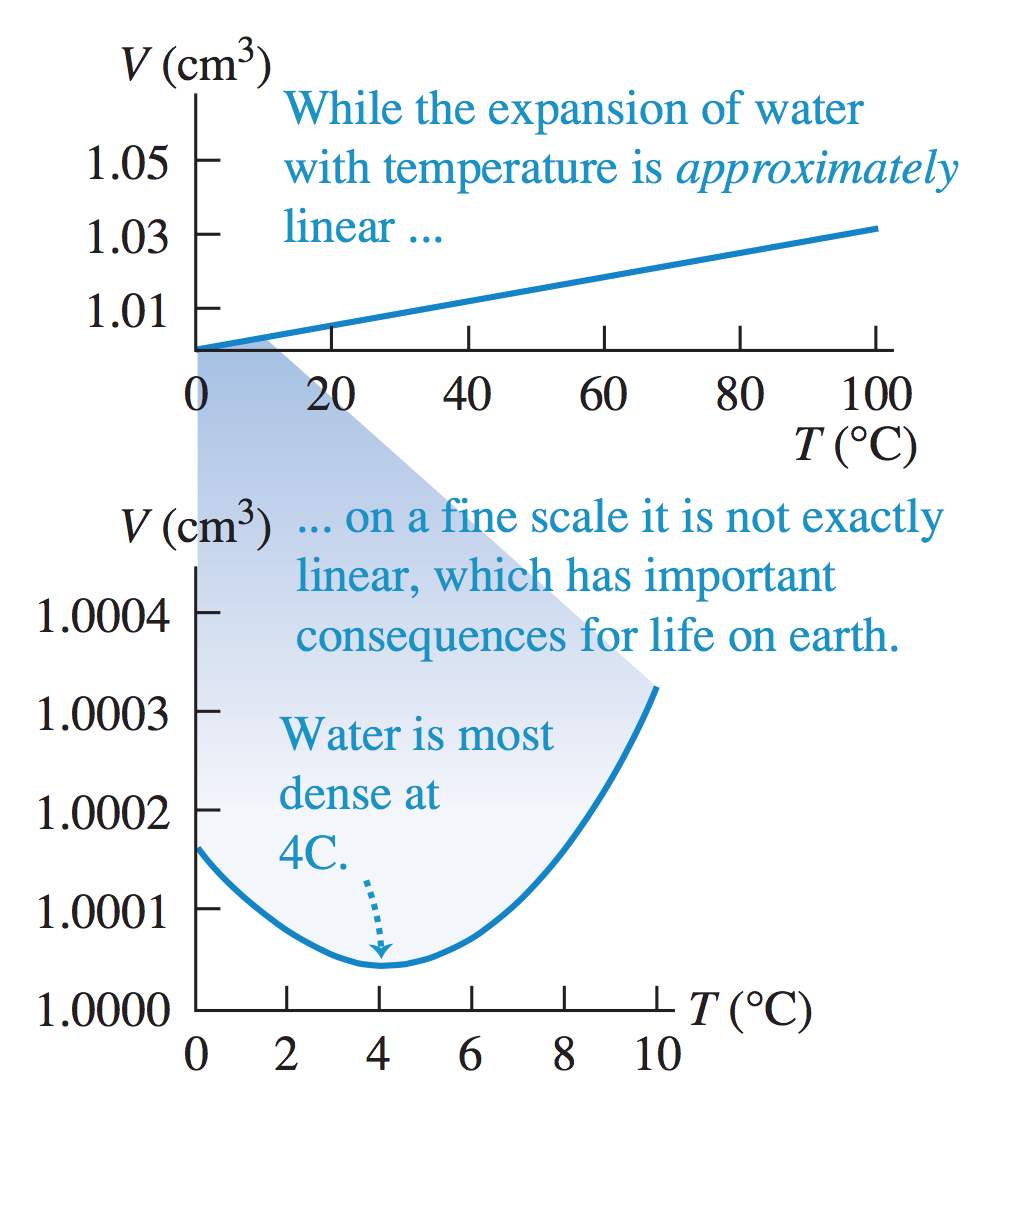
\includegraphics[scale=0.47]{data/img/figure01}
	\caption{El volumen de un gramo de agua a temperatura $T \in [0º, 100º]$, ha aumentado a 1.034 $cm^3$. Si el coeficiente de exoansión del agua fuer constante, se observaría una relación lineal. Imagen tomada de \cite{young2011sears}}
\end{figure}

\begin{itemize}
\item Demostración: (Ver figura 2)

\begin{figure}[htbp]
\centering
	
\includegraphics[scale=0.47]{data/img/figure03}
	\caption{Demostración}
\end{figure}

\item $\alpha = 3.3 \times 10^{-6}\ K^{-1}$ : coeficiente de dilatación lineal del vidrio  
\end{itemize}

\newpage

\section*{Procedimiento experimental}

En este experimento, se busca observar el efecto que tiene la temperatura sobre el volumen de una muestra de agua. El cambio en volumen es pequeño pero lo hacemos visible forzándolo a presentarse en un tubo delgado. Dadas las peculiaridades de la dilatación térmica del agua el modelo lineal no es valido en todo el intervalo de temperaturas que vamos a estudiar, en consecuencia tenemos que tener cuidado de interpretar correctamente las mediciones obtenidas. Los materiales necesarios son:

\begin{itemize}
\item Tubo delgado de vidrio.
\item Tapón
\item Vaso
\item Agua
\item Matraz de Erlenmeyer
\item Termómetro
\item Calibrador
\item Balanza
\item Probeta
\end{itemize}

\begin{figure}[htbp]
\centering
	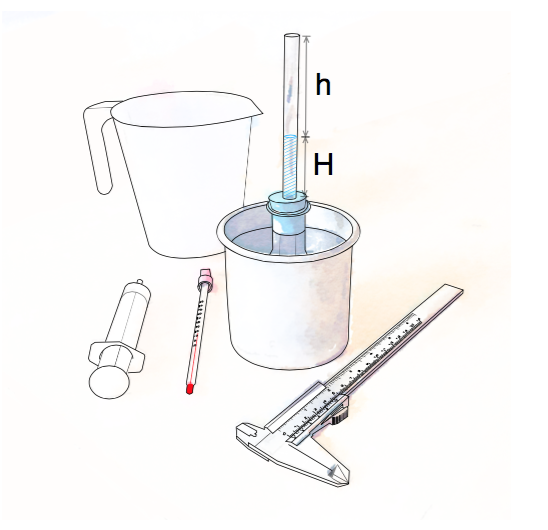
\includegraphics[scale=0.6]{data/img/figure02}
	\caption{Disposición de elementos para el desarrollo del laboratorio.}
\end{figure}

Calentamos agua a una temperatura no inferior a $65º$C. Ponemos el matraz al interior del vaso de aluminio vació y vertimos en el agua caliente hasta que quede completa- mente lleno. Ponemos el tapón (que tiene ajustado el tubo) cuidándonos de que quede muy bien fijo y de que al interior del matraz no queden burbujas de aire. Llenamos completamente el tubo con agua caliente. Llenamos casi completamente el vaso con agua caliente; esta agua que rodea al matraz sirve el propósito de reservorio térmico.\\

Disminuimos la temperatura del reservorio térmico añadiendo agua fría o reemplazando algo del agua del reservorio con agua fría; cambios de temperatura de $5º$C son apropiados. Medimos la temperatura del agua al interior del matraz, como hacer esto?, y tomamos con el calibrador la distancia h (ver figura) que indica el nivel del agua dentro del tubo.\\

Disminuimos repetidamente la temperatura y registramos datos hasta llegar a la temperatura ambiente. Al final, para medir el volumen inicial de la muestra de agua, llenamos el tubo con agua a temperatura ambiente, y con la ayuda de una probeta graduada, o con una balanza, lo determinamos.

\section*{Análisis cualitativo}

\begin{enumerate}
\item Un reservorio térmico, es un recipiente que sirve para reservar las temperaturas sin pérdidas de calor. Uno ideal, no posee el mismo perdidas de calor ni presenta cambios frente la temperatura contenida.

\item El agua expande su volumen para adaptarse a la forma de 
l recipiente ocupado.
\end{enumerate}


%----------------------------------------------------------------------------------------
%	REFERENCE LIST
%----------------------------------------------------------------------------------------

\begin{thebibliography}{99} % Bibliography - this is intentionally simple in this template

  \bibitem{young2011sears} Sears and Zemansky.B. {\em Sears and Zemansky's University Physics / Tutorials in Introductory Physics / Tutorials in Introductory Physics Homework. 17:565--567}, Pearson Education.  2011.
 
\end{thebibliography}

%----------------------------------------------------------------------------------------

\end{document}